\documentclass{standalone}
\usepackage{tikz}
\usepackage{ctex,siunitx}
\usepackage{tkz-euclide}
\usepackage{amsmath}
\usetikzlibrary{patterns, calc}
\usetikzlibrary {decorations.pathmorphing, decorations.pathreplacing, decorations.shapes,}
\begin{document}
\small
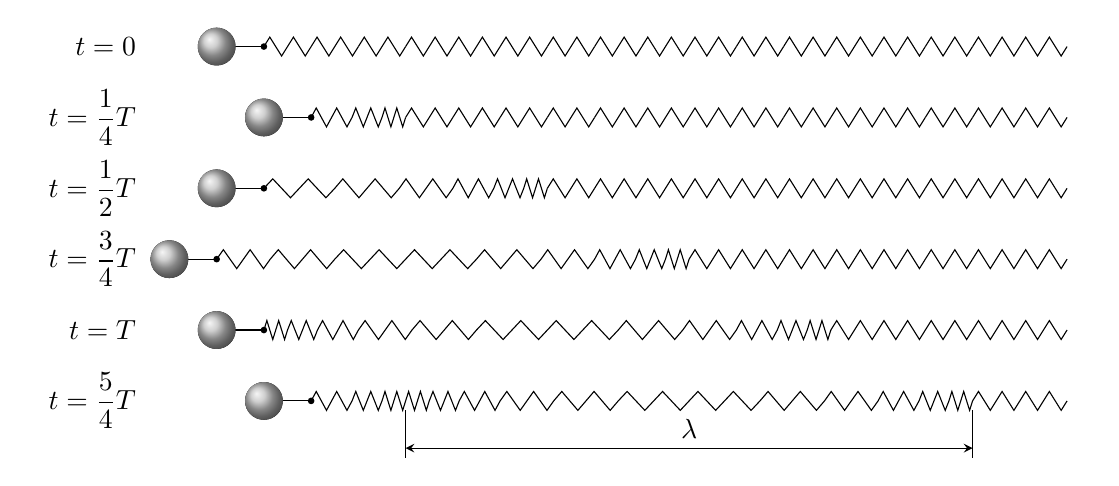
\begin{tikzpicture}[>=stealth,scale=0.6,samples=200]
  \useasboundingbox(-5.0,0.4)rectangle(17.5,-8.7);
  \node at (-2.5,0)[left]{$t=0$};
  \fill(0,0)circle(2pt);
  \draw(0,0)--++(-1,0);
  \fill[ball color=lightgray] (-1,0)circle(0.4);
  \foreach \x in {0,1,...,16}
    { \draw(\x,0)--++(0.125,0.2)--++(0.25,-0.4)--++(0.25,0.4)--++(0.25,-0.4)--++(0.125,0.2); }
  \begin{scope}[yshift=-1.5cm]
    \node at (-2.5,0)[left]{$t=\dfrac{1}{4}T$};
    \fill(1,0)circle(2pt);
    \draw(1,0)--++(-1,0);
    \fill[ball color=lightgray] (0,0)circle(0.4);
    \draw(1.000, 0.0)--(1.108, 0.2)--(1.325,-0.2)--(1.541, 0.2)--(1.758,-0.2)--(1.866, 0.0)--(1.945, 0.2)--(2.104,-0.2)--(2.262, 0.2)--(2.421,-0.2)--(2.500, 0.0)--(2.563, 0.2)--(2.688,-0.2)--(2.813, 0.2)--(2.938,-0.2)--(3.000, 0.0);
    \foreach \x in {3,4,...,16}
      { \draw(\x,0)--++(0.125,0.2)--++(0.25,-0.4)--++(0.25,0.4)--++(0.25,-0.4)--++(0.125,0.2); }
  \end{scope}
  \begin{scope}[yshift=-3cm]
    \node at (-2.5,0)[left]{$t=\dfrac{1}{2}T$};
    \fill(0,0)circle(2pt);
    \draw(0,0)--++(-1,0);
    \fill[ball color=lightgray] (-1,0)circle(0.4);
    \draw(0.000, 0.0)--(0.188, 0.2)--(0.563,-0.2)--(0.938, 0.2)--(1.313,-0.2)--(1.500, 0.0)--(1.671, 0.2)--(2.012,-0.2)--(2.354, 0.2)--(2.695,-0.2)--(2.866, 0.0)--(3.008, 0.2)--(3.291,-0.2)--(3.575, 0.2)--(3.858,-0.2)--(4.000, 0.0)--(4.108, 0.2)--(4.325,-0.2)--(4.541, 0.2)--(4.758,-0.2)--(4.866, 0.0)--(4.945, 0.2)--(5.104,-0.2)--(5.262, 0.2)--(5.421,-0.2)--(5.500, 0.0)--(5.562, 0.2)--(5.687,-0.2)--(5.812, 0.2)--(5.937,-0.2)--(6.000, 0.0);
    \foreach \x in {6,7,...,16}
      { \draw(\x,0)--++(0.125,0.2)--++(0.25,-0.4)--++(0.25,0.4)--++(0.25,-0.4)--++(0.125,0.2); }
  \end{scope}
  \begin{scope}[yshift=-4.5cm]
    \node at (-2.5,0)[left]{$t=\dfrac{3}{4}T$};
    \fill(-1,0)circle(2pt);
    \draw(-1,0)--++(-1,0);
    \fill[ball color=lightgray] (-2,0)circle(0.4);
    \draw(-1.000, 0.0)--(-0.858, 0.2)--(-0.575,-0.2)--(-0.291, 0.2)--(-0.008,-0.2)--( 0.134, 0.0)--( 0.305, 0.2)--( 0.646,-0.2)--( 0.988, 0.2)--( 1.329,-0.2)--( 1.500, 0.0)--( 1.688, 0.2)--( 2.063,-0.2)--( 2.438, 0.2)--( 2.813,-0.2)--( 3.000, 0.0)--( 3.188, 0.2)--( 3.563,-0.2)--( 3.938, 0.2)--( 4.313,-0.2)--( 4.500, 0.0)--( 4.671, 0.2)--( 5.012,-0.2)--( 5.354, 0.2)--( 5.695,-0.2)--( 5.866, 0.0)--( 6.008, 0.2)--( 6.291,-0.2)--( 6.575, 0.2)--( 6.858,-0.2)--( 7.000, 0.0)--( 7.108, 0.2)--( 7.325,-0.2)--( 7.541, 0.2)--( 7.758,-0.2)--( 7.866, 0.0)--( 7.945, 0.2)--( 8.104,-0.2)--( 8.262, 0.2)--( 8.421,-0.2)--( 8.500, 0.0)--( 8.562, 0.2)--( 8.687,-0.2)--( 8.812, 0.2)--( 8.937,-0.2)--( 9.000, 0.0);
    \foreach \x in {9,10,...,16}
      { \draw(\x,0)--++(0.125,0.2)--++(0.25,-0.4)--++(0.25,0.4)--++(0.25,-0.4)--++(0.125,0.2); }
  \end{scope}
  \begin{scope}[yshift=-6cm]
    \node at (-2.5,0)[left]{$t=T$};
    \fill(0,0)circle(2pt);
    \draw(0,0)--++(-1,0);
    \fill[ball color=lightgray] (-1,0)circle(0.4);
    \draw( 0.000, 0.0)--( 0.063, 0.2)--( 0.188,-0.2)--( 0.313, 0.2)--( 0.438,-0.2)--( 0.500, 0.0)--( 0.579, 0.2)--( 0.738,-0.2)--( 0.896, 0.2)--( 1.055,-0.2)--( 1.134, 0.0)--( 1.242, 0.2)--( 1.459,-0.2)--( 1.675, 0.2)--( 1.892,-0.2)--( 2.000, 0.0)--( 2.142, 0.2)--( 2.425,-0.2)--( 2.709, 0.2)--( 2.992,-0.2)--( 3.134, 0.0)--( 3.305, 0.2)--( 3.646,-0.2)--( 3.988, 0.2)--( 4.329,-0.2)--( 4.500, 0.0)--( 4.688, 0.2)--( 5.063,-0.2)--( 5.438, 0.2)--( 5.813,-0.2)--( 6.000, 0.0)--( 6.187, 0.2)--( 6.562,-0.2)--( 6.937, 0.2)--( 7.312,-0.2)--( 7.500, 0.0)--( 7.671, 0.2)--( 8.012,-0.2)--( 8.354, 0.2)--( 8.695,-0.2)--( 8.866, 0.0)--( 9.008, 0.2)--( 9.291,-0.2)--( 9.575, 0.2)--( 9.858,-0.2)--(10.000, 0.0)--(10.108, 0.2)--(10.325,-0.2)--(10.541, 0.2)--(10.758,-0.2)--(10.866, 0.0)--(10.945, 0.2)--(11.104,-0.2)--(11.262, 0.2)--(11.421,-0.2)--(11.500, 0.0)--(11.562, 0.2)--(11.687,-0.2)--(11.812, 0.2)--(11.937,-0.2)--(12.000, 0.0);
    \foreach \x in {12,13,...,16}
      { \draw(\x,0)--++(0.125,0.2)--++(0.25,-0.4)--++(0.25,0.4)--++(0.25,-0.4)--++(0.125,0.2); }
  \end{scope}
  \begin{scope}[yshift=-7.5cm]
    \node at (-2.5,0)[left]{$t=\dfrac{5}{4}T$};
    \fill(1,0)circle(2pt);
    \draw(1,0)--++(-1,0);
    \fill[ball color=lightgray] (0,0)circle(0.4);
    \draw( 1.000, 0.0)--( 1.000, 0.0)--( 1.108, 0.2)--( 1.325,-0.2)--( 1.541, 0.2)--( 1.758,-0.2)--( 1.866, 0.0)--( 1.945, 0.2)--( 2.104,-0.2)--( 2.262, 0.2)--( 2.421,-0.2)--( 2.500, 0.0)--( 2.563, 0.2)--( 2.688,-0.2)--( 2.813, 0.2)--( 2.938,-0.2)--( 3.000, 0.0)--( 3.063, 0.2)--( 3.188,-0.2)--( 3.313, 0.2)--( 3.438,-0.2)--( 3.500, 0.0)--( 3.579, 0.2)--( 3.738,-0.2)--( 3.896, 0.2)--( 4.055,-0.2)--( 4.134, 0.0)--( 4.242, 0.2)--( 4.459,-0.2)--( 4.675, 0.2)--( 4.892,-0.2)--( 5.000, 0.0)--( 5.142, 0.2)--( 5.425,-0.2)--( 5.709, 0.2)--( 5.992,-0.2)--( 6.134, 0.0)--( 6.305, 0.2)--( 6.646,-0.2)--( 6.988, 0.2)--( 7.329,-0.2)--( 7.500, 0.0)--( 7.688, 0.2)--( 8.063,-0.2)--( 8.438, 0.2)--( 8.813,-0.2)--( 9.000, 0.0)--( 9.187, 0.2)--( 9.562,-0.2)--( 9.937, 0.2)--(10.312,-0.2)--(10.500, 0.0)--(10.671, 0.2)--(11.012,-0.2)--(11.354, 0.2)--(11.695,-0.2)--(11.866, 0.0)--(12.008, 0.2)--(12.291,-0.2)--(12.575, 0.2)--(12.858,-0.2)--(13.000, 0.0)--(13.108, 0.2)--(13.325,-0.2)--(13.541, 0.2)--(13.758,-0.2)--(13.866, 0.0)--(13.945, 0.2)--(14.104,-0.2)--(14.262, 0.2)--(14.421,-0.2)--(14.500, 0.0)--(14.562, 0.2)--(14.687,-0.2)--(14.812, 0.2)--(14.937,-0.2)--(15.000, 0.0);
    \foreach \x in {15,16}
      { \draw(\x,0)--++(0.125,0.2)--++(0.25,-0.4)--++(0.25,0.4)--++(0.25,-0.4)--++(0.125,0.2); }
    \draw[thin,<->](3,-1)--(15,-1)node[midway,above]{$\lambda$};
    \draw[thin](3,-0.2)--(3,-1.2)(15,-0.2)--(15,-1.2);
  \end{scope}
\end{tikzpicture}
\end{document}